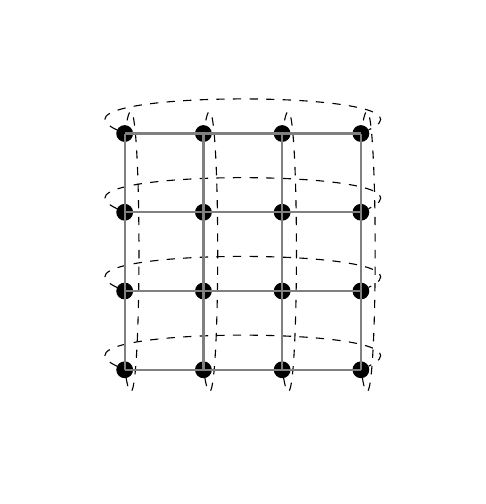
\begin{tikzpicture}

        % First column (tikz has the ability to use loops but I'm drawing it
        % this way so you see how.
        \node (00) [draw, circle, inner sep=2pt,fill] at (0, 0) {};
        \node (01) [draw, circle, inner sep=2pt,fill] at (0, 1) {};
        \node (02) [draw, circle, inner sep=2pt,fill] at (0, 2) {};
        \node (03) [draw, circle, inner sep=2pt,fill] at (0, 3) {};

        % Second column
        \node (10) [draw, circle, inner sep=2pt,fill] at (1, 0) {};
        \node (11) [draw, circle, inner sep=2pt,fill] at (1, 1) {};
        \node (12) [draw, circle, inner sep=2pt,fill] at (1, 2) {};
        \node (13) [draw, circle, inner sep=2pt,fill] at (1, 3) {};

        % Third column
        \node (20) [draw, circle, inner sep=2pt,fill] at (2, 0) {};
        \node (21) [draw, circle, inner sep=2pt,fill] at (2, 1) {};
        \node (22) [draw, circle, inner sep=2pt,fill] at (2, 2) {};
        \node (23) [draw, circle, inner sep=2pt,fill] at (2, 3) {};

        % Fourth column
        \node (30) [draw, circle, inner sep=2pt,fill] at (3, 0) {};
        \node (31) [draw, circle, inner sep=2pt,fill] at (3, 1) {};
        \node (32) [draw, circle, inner sep=2pt,fill] at (3, 2) {};
        \node (33) [draw, circle, inner sep=2pt,fill] at (3, 3) {};


        % I am drawing the periodic boundaries before the rest of the grid
        % so that they appear 'behind' the rest of the images.
        % Draw the period horizontal boundary
        \draw[dashed] (00) to[out=155,in=25 ] (30);
        \draw[dashed] (01) to[out=155,in=25 ] (31);
        \draw[dashed] (02) to[out=155,in=25 ] (32);
        \draw[dashed] (03) to[out=155,in=25 ] (33);

        % Draw the period vertical boundary
        \draw[dashed] (00) to[out=-80,in=80] (03);
        \draw[dashed] (10) to[out=-80,in=80] (13);
        \draw[dashed] (20) to[out=-80,in=80] (23);
        \draw[dashed] (30) to[out=-80,in=80] (33);

        % Draw a grid (this is a tikz shortcut)
        \draw[style=help lines,thick] (0,0) grid  (3,3);
\end{tikzpicture}
